\section{Situando semillas}
Como ya dijimos, la materia gris est\'a compuesta principalmente por neuronas,
y la materia blanca por axones que las comunican. Como cada neurona
posee asociado un ax\'on, colocar semillas en la interfaz entre la materia gris
y la blanca permite caracterizar las neuronas de la corteza \cite{Mori2002}
\cite{Anwander2006}. Cibu et al. \cite{Thomas2014} muestran que la materia blanca
cercana a la materia gris est\'a interconectada por peque\~nos axones. Como
estamos interesados en realizar un estudio de las conexiones entre regiones
distantes del cerebro, decidimos situar las semillas a \textit{3mm} de la corteza,
evitando as\'i el efecto de \'estos axones locales. El problema es que la corteza
del cerebro no es uniforme, sino que est\'a llena de surcos y circunvoluciones. 
Calcular la distancia entonces no es inmediato, necesita un m\'etodo que tome
estas propiedades en cuenta. A continuaci\'on presentamos dos algoritmos: 
erosi\'on binaria y \textit{Fast Marching Method}. Luego, mostramos dos m\'etodos
para posicionar semillas dentro de la materia blanca que utilizan estos algoritmos.
El primer m\'etodo para posicionar semillas es aplicable a cualquier conjunto de
datos, mientras que el segundo aprovecha la informaci\'on disponible de cada sujeto
en \textit{Human Connectome Project}. \\

La erosi\'on binaria es una de las dos operaciones morfol\'ogicas b\'asicas en el
procesamiento de im\'agenes \cite{Serra1983}. Dada una imagen binaria $A$ y una
estructura binaria $B$ se define la erosi\'on $ A \ominus B $ como el proceso
iterativo de centrar la estructura $B$ en cada voxel $v$ que vale uno de $A$, si
existe un elemento superpuesto entre $A$ y $B$ donde $B$ vale uno y $A$ vale cero,
entonces cambiar $v$ a cero. Este proceso posee complejidad $O(\#A\#B)$, donde 
$\#X$ es la cantidad de voxels que posee la imagen $X$.\\

\begin{figure}[h!]

\centering
\begin{minipage}[b]{0.7\textwidth}
    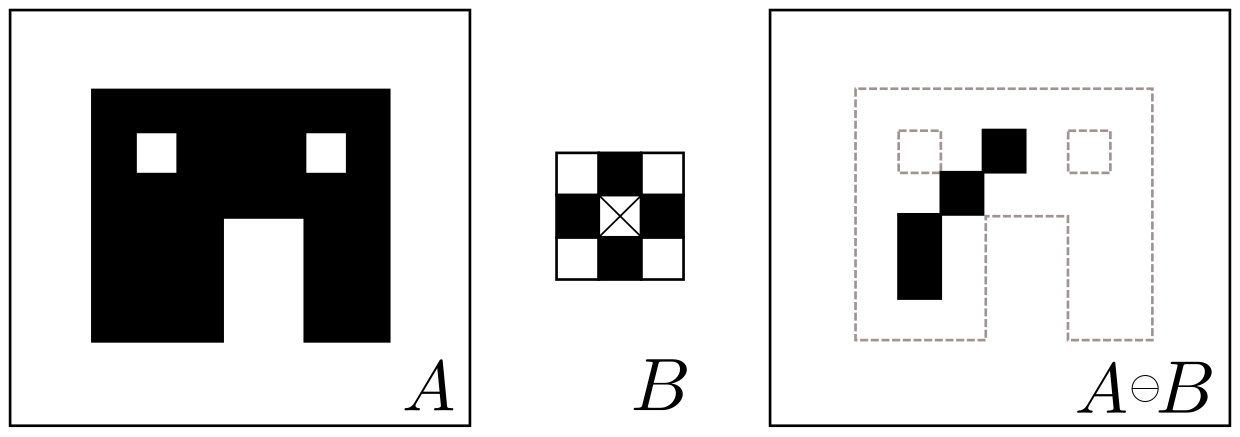
\includegraphics[width=\textwidth]{img/erosion.png}
    \caption{Ejemplo de erosi\'on en imagen binaria}
\end{minipage} ~

\end{figure}  

\textit{Fast Marching Method} es un m\'etodo para resolver num\'ericamente una
versi\'on restringida de la ecuaci\'on \textit{Eikonal}. La misma, en su forma
general, es una ecuaci\'on diferencial no lineal que se encuentra com\'unmente 
en problemas de propagaci\'on de onda. Tiene la forma: 

$$ V(x) | \nabla u(x) | = F(x) , x \in \Omega $$ 

Donde $\Omega$ es un subconjunto abierto de $R^n$ con un
\textit{buen comportamiento} en su borde. $F(x)$ se denomina el costo temporal y
$V(x)$ es la velocidad de la onda en cada punto. En el caso particular que
queremos resolver $u(x_\omega) = 0, x \in \delta\Omega$;  $F(x)=1$ y $V(x)=1$,
por lo que la ecuaci\'on se resume a:

$$ | \nabla u(x) | = 1 , x \in \Omega $$ 

$u(v)$ en este caso representa el tiempo que tarda la onda en llegar desde
alg\'un elemento del borde hasta el punto $v$ movi\'endose a velocidad constante
de una unidad de espacio por unidad de tiempo. Dada la forma de la velocidad, 
$u(v)$ tambi\'en representa \textbf{la distancia mas corta que existe entre cualquier
punto $v$ de la imagen y el borde de $\Omega$}. Dependiendo la orientaci\'on que 
se elija, las distancias a los puntos internos de la superficie ser\'an negativas
y las distancias a los puntos externos positivas (Figura \ref{fig:fmm}). 
\textit{FMM} resuelve este problema en tiempo $O(n log(n))$ \cite{Sethian2001},
siendo $n$ la cantidad de voxels de la imagen.\\

\begin{figure}[h!]

\centering
\begin{minipage}[b]{0.7\textwidth}
    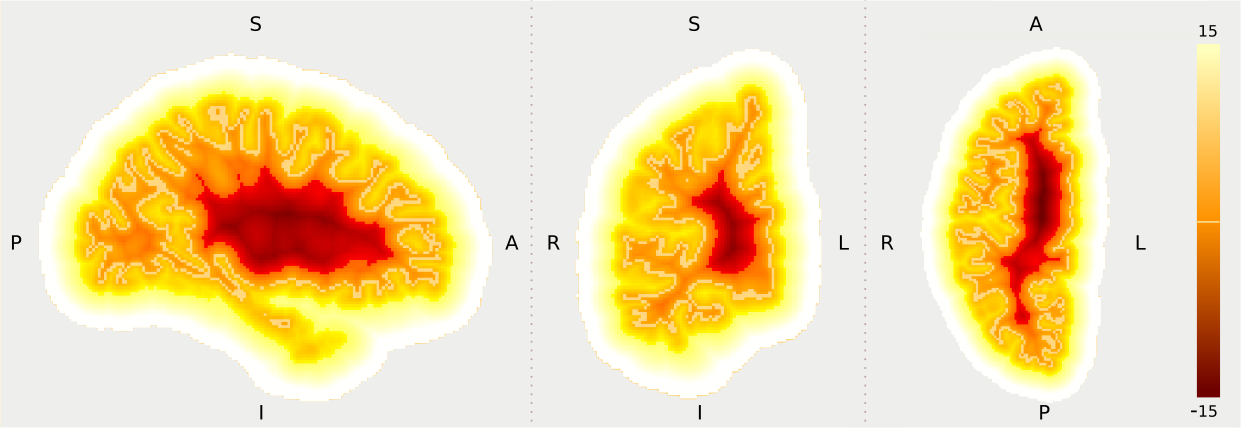
\includegraphics[width=\textwidth]{img/fmm.png}
    \caption{\small FMM sobre el hemisferio derecho, el borde la materia blanca fue
    resaltado intensionalmente}
    \label{fig:fmm}
\end{minipage} ~

\end{figure}  

Una forma de seleccionar voxels para que sean semillas es discriminar la materia
blanca del resto de la imagen; calcular su borde usando erosi\'on binaria; generar
un mapa de distancias con signo desde el borde al resto de la materia blanca usando 
\textit{Fast Marching Method} y seleccionar como semillas los voxels que est\'an
a la distancia deseada. Este m\'etodo puede ser aplicado a cualquier conjunto
de datos y su complejidad es $O(n log(n)) + O(f)$, donde $n$ es la cantidad 
de voxels en la imagen y $f$ es el costo de separar la materia blanca del resto
de la imagen.\\

Recordemos que la finalidad de este trabajo es parcelar la corteza cerebral y 
que para ellos agrupamos los tractogramas de las semillas. Adaptar la selecci\'on
de semillas permite simplificar el proceso de mapear el \textit{clustering} a la 
corteza. Cada sujeto de \textit{HCP} cuenta con un archivo que representa la 
materia gris en forma de superficie. Es posible tomar los puntos definidos en la
superficie y usarlos como borde para calcular el mapa de distancias sobre la 
materia blanca. Caminar desde la corteza siguiendo el gradiente del mapa permite
adentrarse respetando la morfolog\'ia de la materia blanca. La ventaja de este
m\'etodo es que permite guardar un mapeo entre cada coordenada de la superficie y
la semilla que la representa. La complejidad temporal de este m\'etodo es 
$O(n log(n))$. Los sujetos de \textit{HCP} cuentan con una mascara que permite 
discriminar la materia blanca en tiempo lineal. Para mas detalles referirse al Anexo. \\
